\documentclass{beamer}

\usepackage[english]{babel}
\usepackage[utf8x]{inputenc}			
\usepackage{listings}
\usepackage{xcolor}

\lstset{
    language=R,
    basicstyle=\ttfamily\small,
    backgroundcolor=\color{gray!10},
    frame=single,
    breaklines=true,
    showstringspaces=false,
    keywordstyle=\color{blue},
    commentstyle=\color{green!50!black},
    stringstyle=\color{red},
    numbers=none,
    xleftmargin=10pt,
    xrightmargin=10pt,
    framexleftmargin=5pt,
    framexrightmargin=5pt
}

\mode<presentation>						
{
  \usetheme{default}					
  \usecolortheme{default} 			
  \usefonttheme{default}  				
  \setbeamertemplate{caption}[numbered]	
}

\usepackage{graphicx}
\graphicspath{{figure/}}				% Shared figure folder for all labs
\usepackage{booktabs}
\usepackage{hyperref}					
\usepackage{subcaption}  
\usepackage{multicol}
\usepackage{hyperref}

\title{Probability Distribution}	
\author{Rex Shao-Yu Wang}								
\institute{Department of Agronomy, National Taiwan University}				
\date{March 30, 2026}								

\begin{document}

% Title page
\begin{frame}
  \titlepage
\end{frame}

% Outline
\begin{frame}{Outline}
  \tableofcontents
\end{frame}

\section{Binomial Distribution}
\begin{frame}[fragile]{Math Calculation}
\begin{itemize}
    \item \textbf{Combination:} $C^{n}_{k}$ or $\binom{n}{k}$\\
    \vspace{5pt}
    $choose(n, k) = \binom{n}{k} = \frac{n!}{k! (n-k)!}$
    \vspace{5pt}
    \begin{lstlisting}
        choose(5, 3)
    \end{lstlisting}
    \vspace{10pt}
    \item \textbf{Factorial:} $x!$\\
    \vspace{5pt}
    $factorial(x) = x! = 1\times2\times\cdots\times(x-1)\times x$
    \vspace{5pt}
    \begin{lstlisting}
        factorial(10)
    \end{lstlisting}
\end{itemize}

    
\end{frame}
\begin{frame}{Binomial Distribution}
\begin{center}
    {\LARGE $X \sim Bin(n, p) $}
\end{center}
\textbf{X} : The number of successes in n independent Bernoulli trials \\
\textbf{n} : Fixed number of independent trials \\
\textbf{p} : Constant probability of success in each trial\\
\vspace{10pt}
Probability Mass Function: 
\begin{equation}
P(X = x) = \binom{n}{x} \times p^x\times (1-p)^{n-x}
\end{equation}\\
Mean and Variance:
\begin{center}
$\mu = np$, $\sigma^2 = np(1-p)$
\end{center}
\end{frame}

\begin{frame}[fragile]{dbinom(x, n = size, p = prob)}
Returns the value of the probability when X = x\\
\vspace{10pt}
Example:\\
\begin{enumerate}
    \item $X \sim Bin(20, 0.6)$. Try to find $P(X = 5)$ ?
    \begin{lstlisting}
    dbinom(x = 5, n = 20, p = 0.6)
    \end{lstlisting}
    \item $X \sim Bin(10, 0.3)$. Try to find $P(4 \le X \le 7)$ ? 
    \begin{lstlisting}
    dbinom(x = 4:7, n = 10, p = 0.7)
    \end{lstlisting}
\end{enumerate}
\begin{figure}
    \centering
    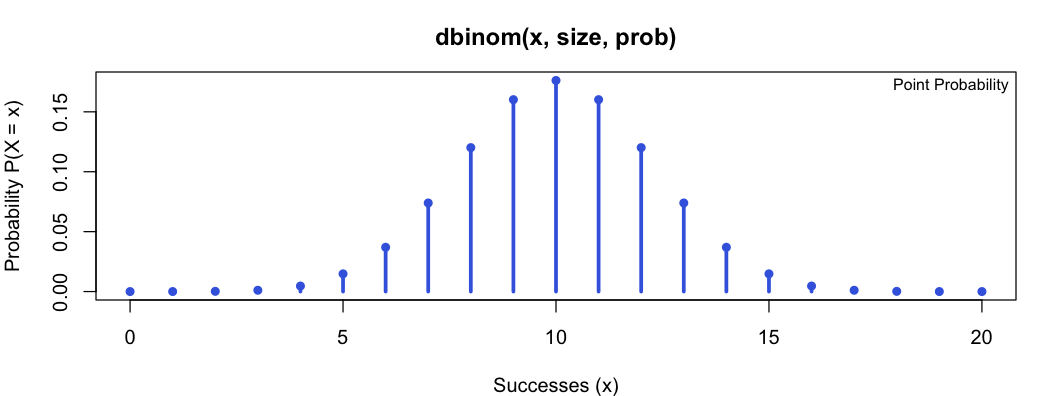
\includegraphics[width=1\linewidth]{dbinom.png}
\end{figure}
\end{frame}

\begin{frame}[fragile]{Cumulative Distribution and Quantiles}
\begin{itemize}
    \item \texttt{pbinom(q, size, prob)}: $P(X \le q)$
    \item \texttt{pbinom(q, size, prob, lower.tail = F)}: $P(X \ge q)$
    \item \texttt{qbinom(p, size, prob)}: \\
    The smallest $x$ such that $P(X \le x) \ge p$ (\textbf{Quantile}).
\end{itemize}
\textbf{Example:}
\begin{lstlisting}
# Find P(X <= 15)
pbinom(q = 15, size = 20, prob = 0.6)
# Find 90th percentile
qbinom(p = 0.9, size = 20, prob = 0.6)
\end{lstlisting}
\begin{figure}
    \centering
    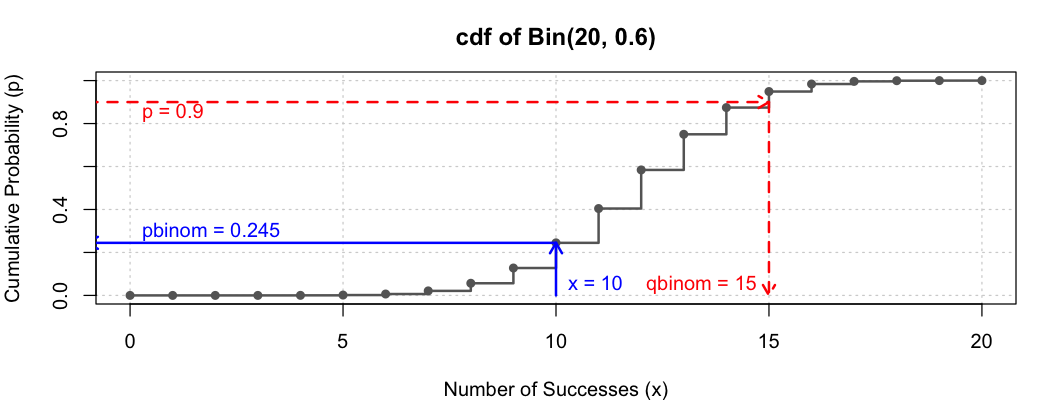
\includegraphics[width=\linewidth]{cdf_binom.png}
\end{figure}
\end{frame}

\begin{frame}[fragile]{rbinom(n, size, prob)}
 Generates $n$ random samples following the binomial distribution $Bin(\text{size}, \text{prob})$
 \vspace{8pt}
\begin{columns}[T]
\begin{column}{0.48\textwidth}
\textbf{Example:}
\begin{lstlisting}[language=R, basicstyle=\scriptsize\ttfamily, xleftmargin=0.5em]
# Generate 100 samples
rbinom(100, size = 20, prob = 0.5)

# Visualize different sample sizes
hist(rbinom(100, 20, 0.5), 
     main = "n = 100")
hist(rbinom(1000, 20, 0.5), 
     main = "n = 1000")
hist(rbinom(10000, 20, 0.5), 
     main = "n = 10000")
\end{lstlisting}
\end{column}
        
\begin{column}{0.48\textwidth}
\begin{figure}
    \centering
    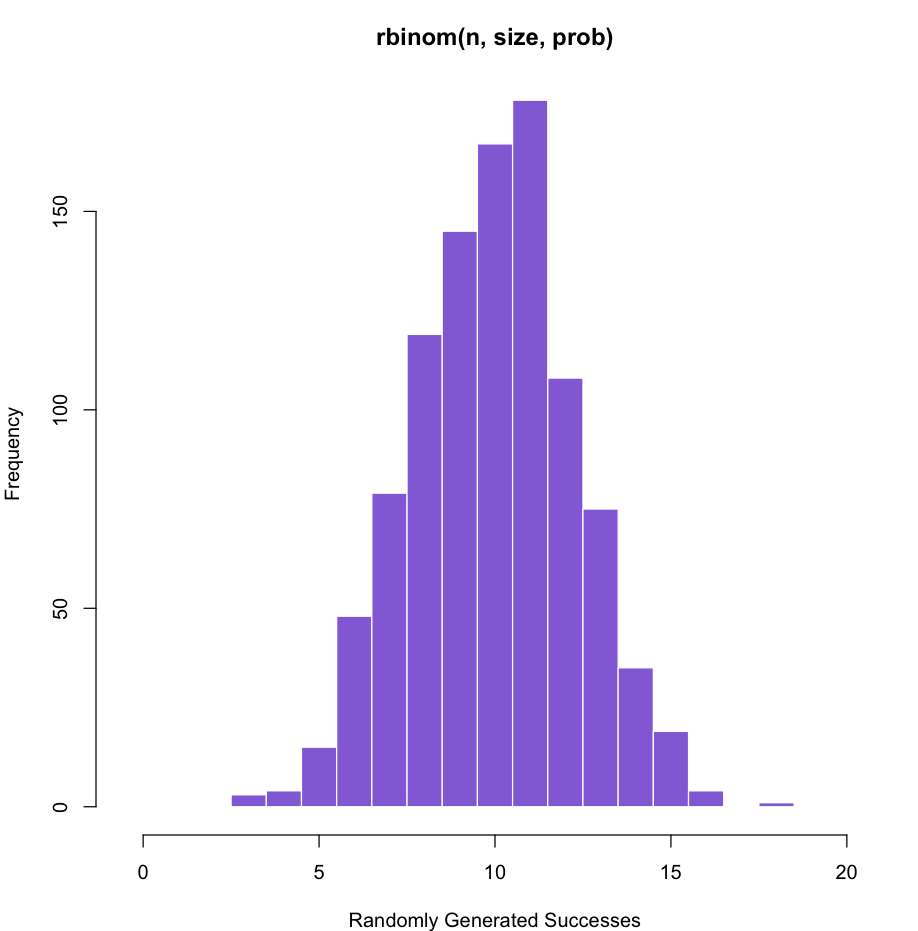
\includegraphics[width=1.2\linewidth]{rbinom.png}
\end{figure}
\end{column}

\end{columns}
\end{frame}


\section{Poisson Distribution}
\begin{frame}{Poisson Distribution}
\begin{center}
    {\LARGE $X \sim Poisson(\lambda) $}
\end{center}
\textbf{X} : The count of rare events within a specific time or space interval\\
\textbf{$\lambda$} : The average number of occurrences per interval \\
\vspace{10pt}
Probability Mass Function: 
\begin{equation}
P(X = x) = \frac{\lambda^{x}e^{-\lambda}}{x!}
\end{equation}\\
Mean and Variance:
\begin{center}
$\mu = \lambda$, $\sigma^2 = \lambda$
\end{center}
\end{frame}

\begin{frame}[fragile]{dpois(q, lambda)}
This function returns the value of the Poisson pmf when X = \textbf{q}\\
\vspace{5pt}
\textbf{Example:} We'll use the example in Steven's lecture\\
\vspace{5pt}
Random variable \textbf{X}: Number of snails in a 1-hectare field.\\
On average, there are 1.5 snails per hectare. $\to$ $\lambda= 1.5$\\
What is the probability that there are NO snails (i.e., x = 0)?\\
\vspace{5pt}
\textbf{Answer:}\\
We want to find $P(X = 0)$ when $X \sim Poisson(\lambda = 1.5)$
\begin{lstlisting}
dpois(q = 0, lambda = 1.5)
\end{lstlisting}
\begin{figure}
    \centering
    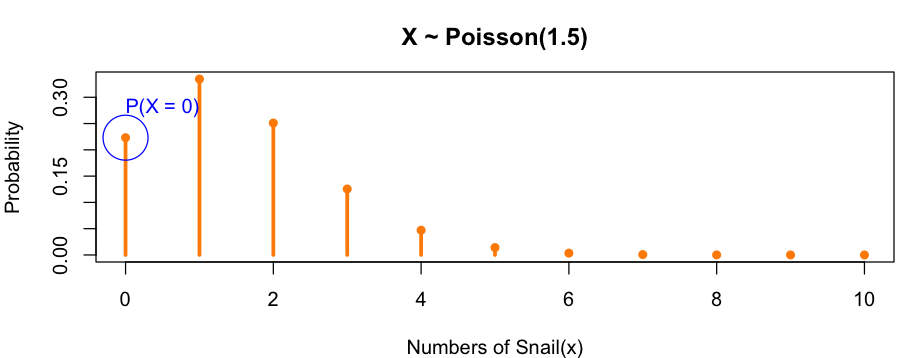
\includegraphics[width=0.88\linewidth]{dpois.png}
\end{figure}
\end{frame}

\begin{frame}[fragile]{ppois(q ,lambda)}
Return the cumulative probability when X = q. (i.e. $P(X \le q)$)\\
\vspace{10pt}
\textbf{Example:}\\
What is the probability that there will be at least one snails?\\
\vspace{5pt}
\textbf{Answer:}\\
We can do this question in two ways: $P(X \ge 1)$ or $1 - P(X \le 1)$
\begin{lstlisting}
# P >= 1
ppois(q=1, lambda=1.5, lower.tail=FALSE)

# p <= 1
1 - ppois(q=1, lambda=1.5)
\end{lstlisting}
\end{frame}

\begin{frame}[fragile]{qpois(p, lambda)}
Number of events that corresponds to a certain percentile(p)\\
Inverse function for ppois()\\
\begin{lstlisting}
x <- ppois(q = 1, lambda = 1.5) 
qpois(p = x, lambda = 1.5)
\end{lstlisting}
\begin{figure}
    \centering
    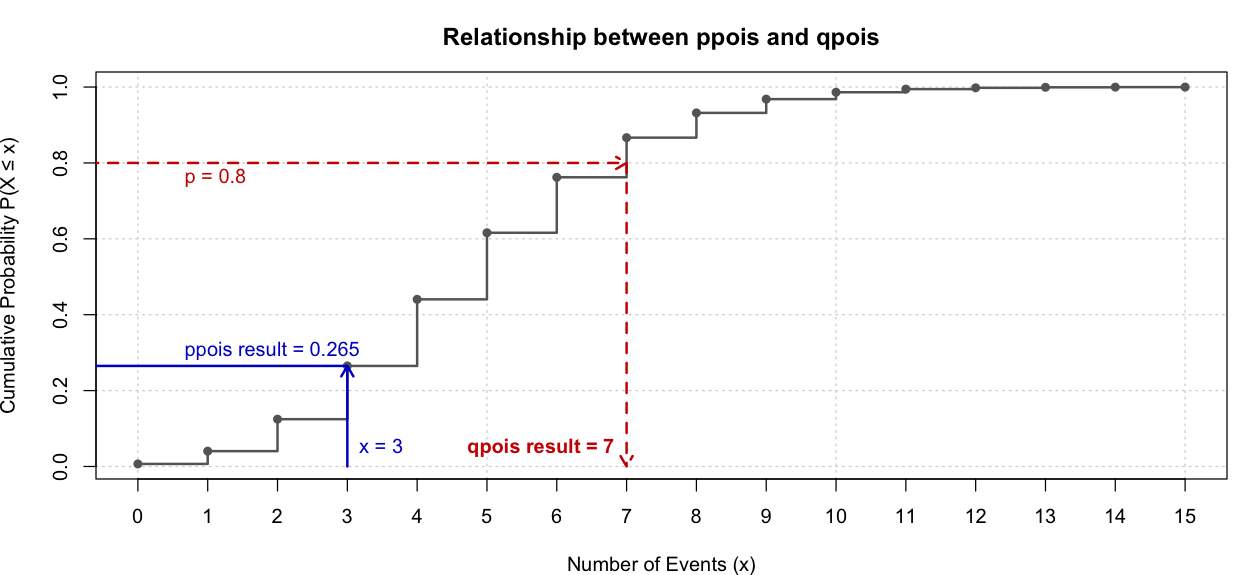
\includegraphics[width=1\linewidth]{pqpois.png}
\end{figure}
\end{frame}

\begin{frame}[fragile]{rpois(n, lambda)}
 Generates $n$ random samples following the Poisson distribution $Poisson(\lambda)$
 \vspace{8pt}
\begin{columns}[T]
\begin{column}{0.48\textwidth}
\textbf{Example:}
\begin{lstlisting}[language=R, basicstyle=\scriptsize\ttfamily, xleftmargin=0.5em]
# Generate 10 samples
rpois(10, 4)

# Visualize different sample sizes
hist(rpois(10, 4), main = "X ~ Poisson(n = 10, lambda = 4)")
hist(rpois(100, 4), main = "X ~ Poisson(n = 100, lambda = 4)")
hist(rpois(1000, 4), main = "X ~ Poisson(n = 1000, lambda = 4)")
hist(rpois(10000, 4), main = "X ~ Poisson(n = 10000, lambda = 4)")
\end{lstlisting}
\end{column}

\begin{column}{0.48\textwidth}
\begin{figure}
    \centering
    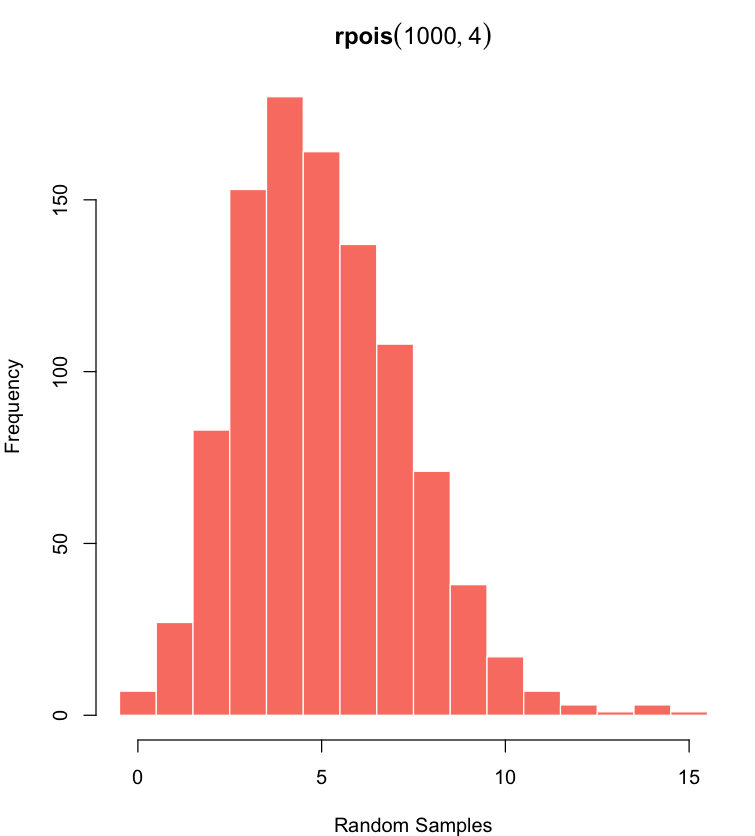
\includegraphics[width=1.1\linewidth]{rpois.png}
\end{figure}
\end{column}

\end{columns}
\end{frame}

\section{Normal Distribution}
\begin{frame}{Normal Distribution}
\begin{center}
    {\LARGE $X \sim \mathcal{N}(\mu, \sigma^2) $}
\end{center}
\textbf{X} : The continuous random variable that follows the normal distribution\\
\textbf{$\mu$ (Mean)} : Defines the center of the distribution \\
\textbf{$\sigma^2$ (Variance)} : Defines the spread or width of the curve\\
\vspace{10pt}
Probability Density Function: 
\begin{equation}
f(x) = \frac{1}{\sqrt{2\pi\sigma^2}} e^{\frac{-(x-\mu)^2}{2\sigma^2}}
\end{equation}\\
Mean and Variance:
\begin{center}
$\mu = \mu$, $\sigma^2 = \sigma^2$
\end{center}
\end{frame}

\begin{frame}[fragile]{dnorm(x, mean, sd)}
\begin{alertblock}{Warning: Density $\neq$ Probability}
        For a continuous variable, the probability of any specific point is \textbf{0}:
        \[ P(X = x) = 0 \]
        \texttt{dnorm()} gives the \textbf{height} of the curve, not the probability!
    \end{alertblock}
\begin{lstlisting}
dnorm(0) # Default: mean = 0, sd = 1
dnorm(1, mean = 2, sd = 3)
\end{lstlisting}
\begin{figure}
    \centering
    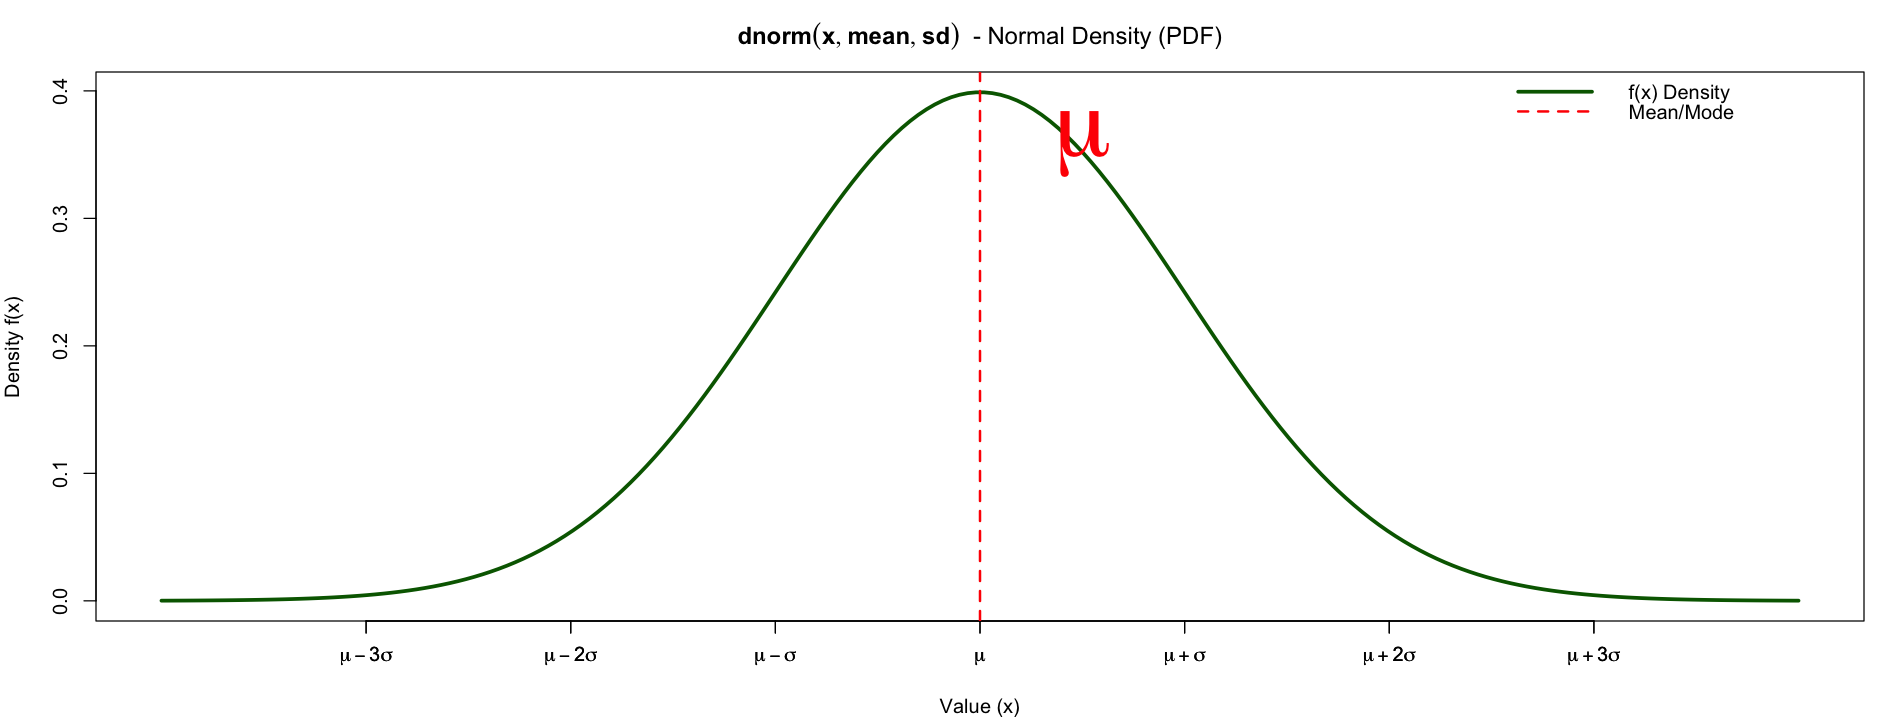
\includegraphics[width=1\linewidth]{dnorm.png}
\end{figure}
\end{frame}

\begin{frame}[fragile]{pnorm(q, mean, sd, lower.tail)}
Return the cumulative probability when X = q. (i.e. $P(X \le q)$)\\
\vspace{10pt}
\textbf{Example:}\\
The size of the corn is normally distributed with a mean of 20cm and a variance of $16 cm^2$. What is the probability that a farmer harvests a corn that is above 26cm? \\
\vspace{5pt}
\textbf{Answer:}\\
Let $X \sim \mathcal{N}(20, 16)$, calculate $P(X \ge 26)$\\
\begin{lstlisting}
# Use P(X >= 26)
pnorm(q = 26, mean = 20, sd = 4, lower.tail = FALSE)

# Use 1 - P(X <= 26)
1 - pnorm(26, 20, 4)
\end{lstlisting}
\end{frame}

\begin{frame}[fragile]{qnorm(p, mean, sd, lower.tail)}

\begin{lstlisting}
qnorm(0.95, mean=0, sd=1)
\end{lstlisting}
\begin{figure}
    \centering
    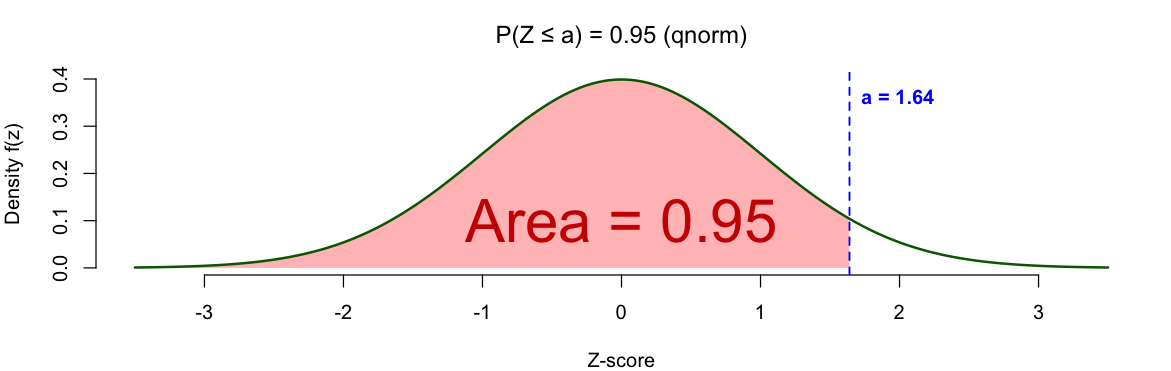
\includegraphics[width=0.9\linewidth]{qnorm.png}
\end{figure}

\begin{lstlisting}
qnorm(0.95, mean=0, sd=1, lower.tail = FALSE)
\end{lstlisting}
\begin{figure}
    \centering
    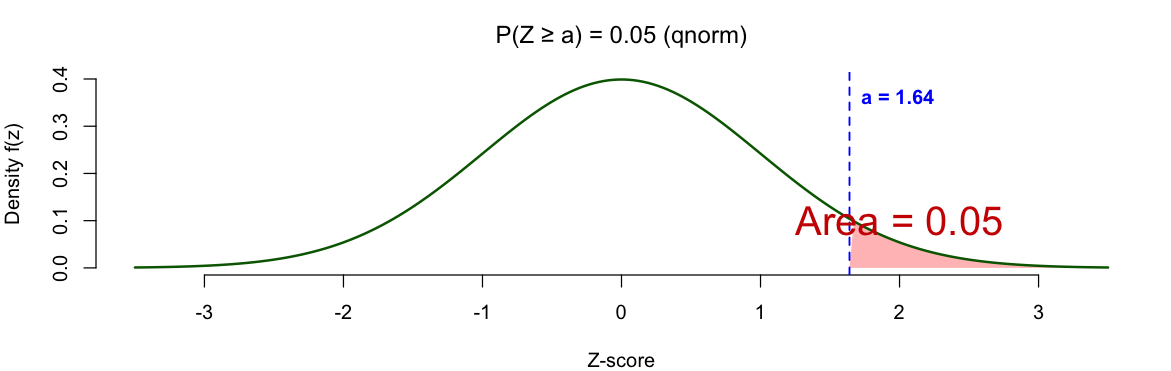
\includegraphics[width=0.9\linewidth]{qnorm(lower.tail).png}
\end{figure}
\end{frame}

\begin{frame}[fragile]{rnorm(n, mean, variance)}
 Generates $n$ random samples following the Normal distribution $N(\mu, \sigma^2)$
 \vspace{8pt}
\begin{columns}[T]
\begin{column}{0.48\textwidth}
\textbf{Example:}
\begin{lstlisting}[language=R, basicstyle=\scriptsize\ttfamily, xleftmargin=0.5em]
# Generate 10000 samples with different mean and variance
rnorm(10000, mean = 0, sd = 1)
rnorm(10000, mean = 5, sd = 0.5)
rnorm(10000, mean = 2, sd = 3)

\end{lstlisting}
\end{column}

\begin{column}{0.48\textwidth}
\begin{figure}
    \centering
    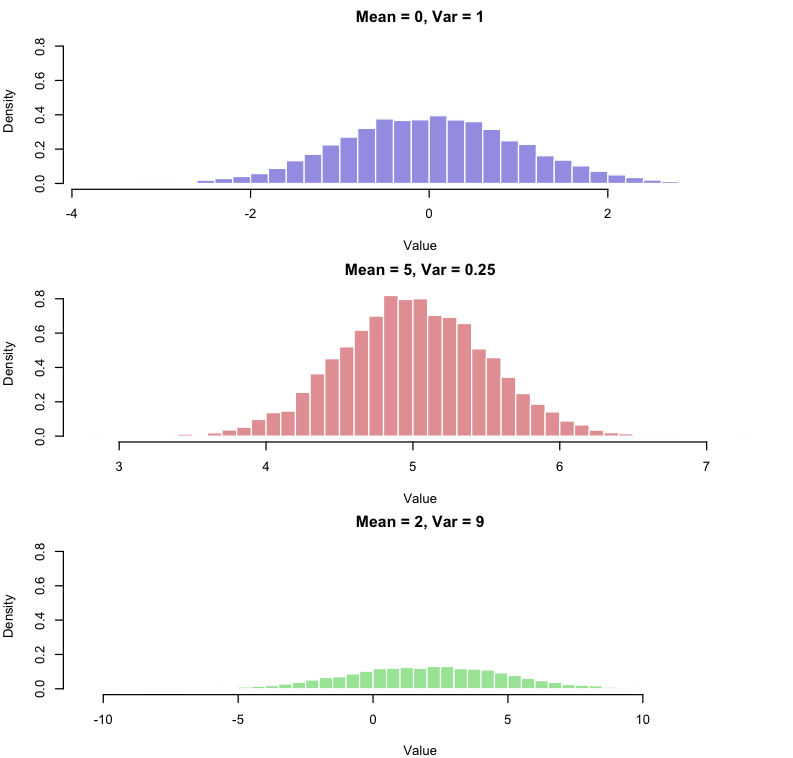
\includegraphics[width=1.3\linewidth]{rnorm.png}
\end{figure}
\end{column}
\end{columns}
\end{frame}

\section{Practice \& Lab Report}
\begin{frame}{Practice}
\begin{enumerate}
\item In how many ways can we select a team of 5 students from a given choice of 20?
\item If a coin is tossed 3 times, then find the probability of getting exactly two heads.
\item An average of 0.61 soldiers died by horse kicks per year in each Prussian army corps. You want to calculate the probability that exactly two soldiers died in the VII Army Corps in 1898, assuming that the number of horse kick deaths per year follows a Poisson distribution.
\item Most graduate schools of business require applicants for admission to take the Graduate Management
Admission Council’s GMAT examination. Scores on the GMAT are roughly normally distributed with a
mean of 527 and a standard deviation of 112. What is the probability of an individual scoring above 500 on
the GMAT? 


\end{enumerate}
\end{frame}

\begin{frame}{Lab Report}
\begin{itemize}
    \item The report file will be in the NTU COOL Assignment section
    \item Submit your file in pdf format
    \item Deadline: 4/5 (Sun) 23:59
    \item Late submission is not accepted
\end{itemize}
\end{frame}
\end{document}

